\documentclass[tikz,border=12pt]{standalone}
\usepackage[T1]{fontenc}
\usepackage{mathpazo}
\usepackage{amsmath,amssymb}
\usetikzlibrary{arrows.meta, positioning, calc, fit, decorations.pathreplacing, patterns}
\usepackage{pgfplots}
\pgfplotsset{compat=1.18}

\definecolor{stblue}{HTML}{7B97AD}
\definecolor{rwgold}{HTML}{B8995E}
\definecolor{sage}{HTML}{7A9A7E}
\definecolor{dkbrown}{HTML}{3D3530}
\definecolor{wmgray}{HTML}{7B7067}
\definecolor{cream}{HTML}{F9F6F0}
\definecolor{border}{HTML}{D4C9B8}
\definecolor{terracotta}{HTML}{C47A6A}
\definecolor{lavender}{HTML}{907EA0}

\begin{document}
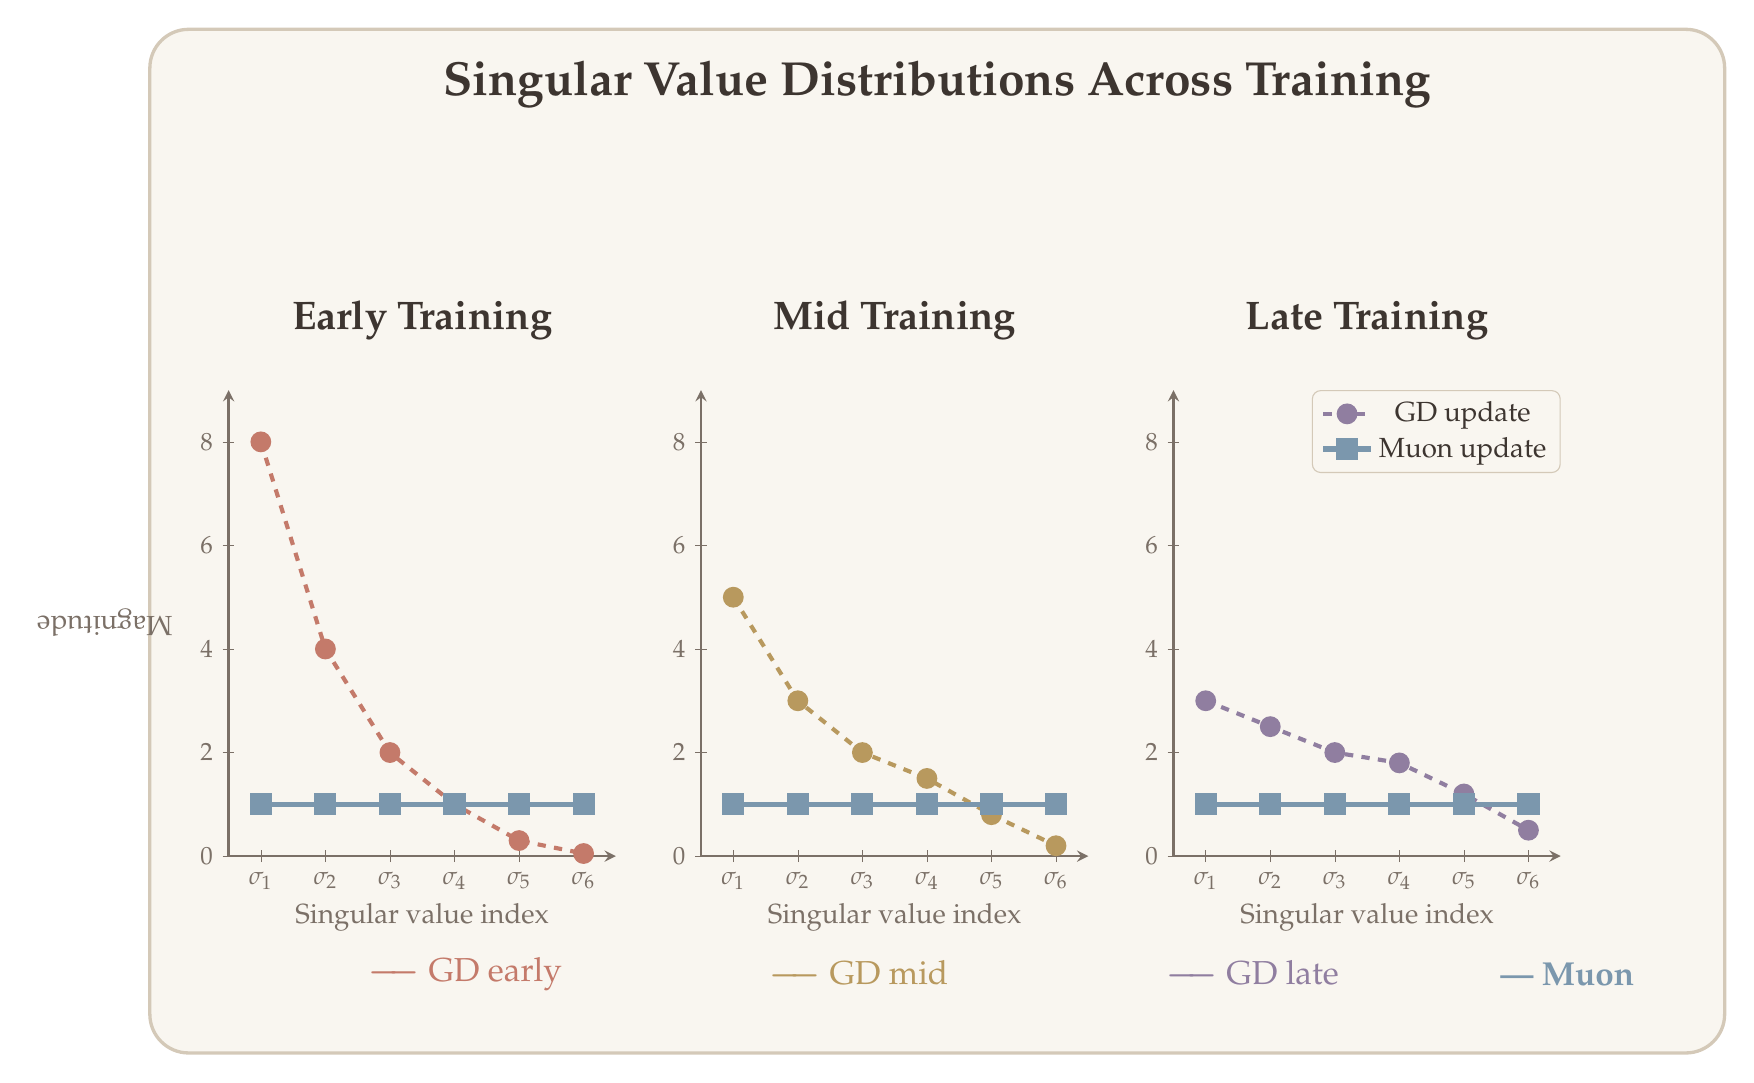
\begin{tikzpicture}[>={Stealth[length=4mm, width=3mm]}, line width=1.5pt]

% Background
\fill[cream, rounded corners=14pt] (-1.0,-2.5) rectangle (19.0,10.5);
\draw[border, line width=1.2pt, rounded corners=14pt] (-1.0,-2.5) rectangle (19.0,10.5);

% Title
\node[text=dkbrown, font=\LARGE\bfseries] at (9.0,9.8) {Singular Value Distributions Across Training};

% ============================================================
% Panel 1: Early Training
% ============================================================
\begin{axis}[
  at={(0.0cm,0.0cm)},
  width=6.5cm,
  height=7.5cm,
  axis lines=left,
  axis line style={wmgray, line width=0.8pt},
  title={\textbf{Early Training}},
  title style={text=dkbrown, font=\Large, at={(0.5,1.05)}},
  xlabel={Singular value index},
  xlabel style={text=wmgray, font=\normalsize, at={(axis description cs:0.5,-0.08)}},
  ylabel={Magnitude},
  ylabel style={text=wmgray, font=\normalsize, at={(axis description cs:-0.12,0.5)}, rotate=90},
  xmin=0.5, xmax=6.5,
  ymin=0, ymax=9,
  xtick={1,2,3,4,5,6},
  xticklabels={$\sigma_1$,$\sigma_2$,$\sigma_3$,$\sigma_4$,$\sigma_5$,$\sigma_6$},
  ytick={0,2,4,6,8},
  tick label style={text=wmgray, font=\small},
  tick style={wmgray},
  axis background/.style={fill=cream},
  clip=false,
]
% GD Early: [8,4,2,1,0.3,0.05]
\addplot[terracotta, dashed, line width=1.5pt, mark=*, mark size=3pt, mark options={solid, fill=terracotta}]
  coordinates {(1,8) (2,4) (3,2) (4,1) (5,0.3) (6,0.05)};

% Muon: [1,1,1,1,1,1]
\addplot[stblue, solid, line width=2pt, mark=square*, mark size=3pt, mark options={solid, fill=stblue}]
  coordinates {(1,1) (2,1) (3,1) (4,1) (5,1) (6,1)};
\end{axis}

% ============================================================
% Panel 2: Mid Training
% ============================================================
\begin{axis}[
  at={(6.0cm,0.0cm)},
  width=6.5cm,
  height=7.5cm,
  axis lines=left,
  axis line style={wmgray, line width=0.8pt},
  title={\textbf{Mid Training}},
  title style={text=dkbrown, font=\Large, at={(0.5,1.05)}},
  xlabel={Singular value index},
  xlabel style={text=wmgray, font=\normalsize, at={(axis description cs:0.5,-0.08)}},
  xmin=0.5, xmax=6.5,
  ymin=0, ymax=9,
  xtick={1,2,3,4,5,6},
  xticklabels={$\sigma_1$,$\sigma_2$,$\sigma_3$,$\sigma_4$,$\sigma_5$,$\sigma_6$},
  ytick={0,2,4,6,8},
  tick label style={text=wmgray, font=\small},
  tick style={wmgray},
  axis background/.style={fill=cream},
  clip=false,
]
% GD Mid: [5,3,2,1.5,0.8,0.2]
\addplot[rwgold, dashed, line width=1.5pt, mark=*, mark size=3pt, mark options={solid, fill=rwgold}]
  coordinates {(1,5) (2,3) (3,2) (4,1.5) (5,0.8) (6,0.2)};

% Muon: [1,1,1,1,1,1]
\addplot[stblue, solid, line width=2pt, mark=square*, mark size=3pt, mark options={solid, fill=stblue}]
  coordinates {(1,1) (2,1) (3,1) (4,1) (5,1) (6,1)};
\end{axis}

% ============================================================
% Panel 3: Late Training
% ============================================================
\begin{axis}[
  at={(12.0cm,0.0cm)},
  width=6.5cm,
  height=7.5cm,
  axis lines=left,
  axis line style={wmgray, line width=0.8pt},
  title={\textbf{Late Training}},
  title style={text=dkbrown, font=\Large, at={(0.5,1.05)}},
  xlabel={Singular value index},
  xlabel style={text=wmgray, font=\normalsize, at={(axis description cs:0.5,-0.08)}},
  xmin=0.5, xmax=6.5,
  ymin=0, ymax=9,
  xtick={1,2,3,4,5,6},
  xticklabels={$\sigma_1$,$\sigma_2$,$\sigma_3$,$\sigma_4$,$\sigma_5$,$\sigma_6$},
  ytick={0,2,4,6,8},
  tick label style={text=wmgray, font=\small},
  tick style={wmgray},
  axis background/.style={fill=cream},
  clip=false,
  legend style={
    at={(1.0,1.0)},
    anchor=north east,
    draw=border,
    fill=cream,
    font=\normalsize,
    text=dkbrown,
    rounded corners=3pt,
  },
]
% GD Late: [3,2.5,2,1.8,1.2,0.5]
\addplot[lavender, dashed, line width=1.5pt, mark=*, mark size=3pt, mark options={solid, fill=lavender}]
  coordinates {(1,3) (2,2.5) (3,2) (4,1.8) (5,1.2) (6,0.5)};
\addlegendentry{GD update}

% Muon: [1,1,1,1,1,1]
\addplot[stblue, solid, line width=2pt, mark=square*, mark size=3pt, mark options={solid, fill=stblue}]
  coordinates {(1,1) (2,1) (3,1) (4,1) (5,1) (6,1)};
\addlegendentry{Muon update}
\end{axis}

% Stage color legend for GD lines
\node[text=terracotta, font=\large] at (3.0,-1.5) {$\boldsymbol{-\!\!-}$ GD early};
\node[text=rwgold, font=\large] at (8.0,-1.5) {$\boldsymbol{-\!\!-}$ GD mid};
\node[text=lavender, font=\large] at (13.0,-1.5) {$\boldsymbol{-\!\!-}$ GD late};
\node[text=stblue, font=\large\bfseries] at (17.0,-1.5) {\textemdash\ Muon};

\end{tikzpicture}
\end{document}
